\chapter{FUNDAMENTAÇÃO TEÓRICA}
\label{chap:fundamentacao-teorica}

% introdução histórica

% não fazer citações diretas. Entender e dar o entendimento

O cimento é composto por uma mistura de calcário e argila, sendo representado por 75-80\% e 20-25\%, respectivamente de cada composto \cite{Andre2011}. Suas aplicações são extremamente difundidas em toda a sociedade, desde a sua invenção, até os dias de hoje. Isso se evidencia quando observamos que a origem do cimento ocorreu há cerca de 4.500 anos. Naquela época, os monumentos do Egito antigo já utilizavam uma liga constituída por uma mistura de gesso calcinado. As grandes obras gregas e romanas, como o Panteão e o Coliseu, foram construídas com o uso de solos de origem vulcânica da ilha grega de Santorino, ou das proximidades da cidade italiana de Pozzuoli, que possuíam propriedades de endurecimento sob a ação da água.\cite{ABCP}. 

 	\begin{figure}[h!] 
   	    \captionsetup{width=16cm}%Da mesma largura que a figura
		\Caption{\label{fig:coliseu} Fotografia do Coliseu, em Roma.}
		\UFCfig{}{
			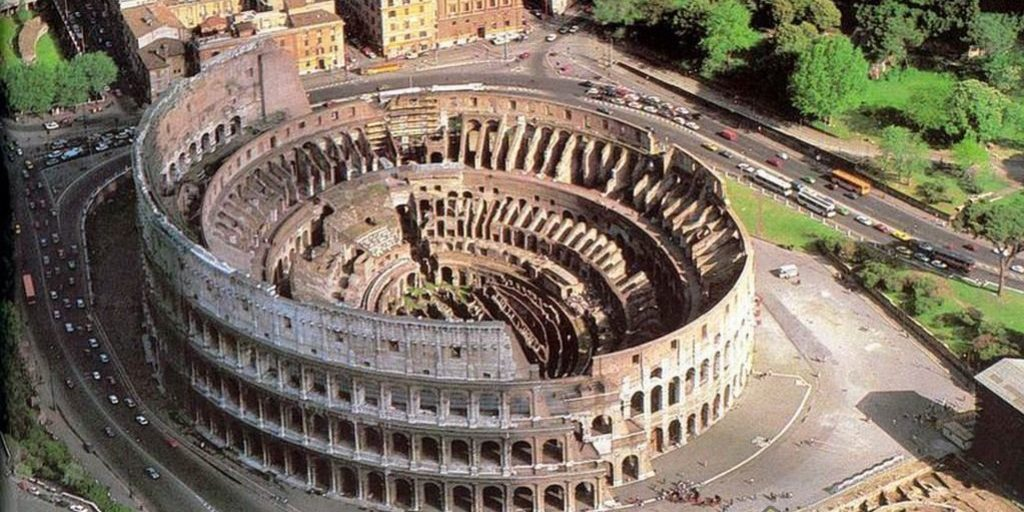
\includegraphics[width=16cm]{figuras/coliseu}
		}{
			\Fonte{\citeonline{Teste2021}.}
		}	
	\end{figure}

Dito isso, o ponto de inflexão no processo de desenvolvimento do cimento aconteceu em 1756 pelo inglês John Smeaton, que através da calcinação de calcários moles e argilosos conseguiu obter um produto resistente. Em 1824, o construtor inglês Joseph Aspdin queimou pedras calcárias e argila, transformando-as num pó fino. A mistura obtida, após secar, tornou-se tão dura quanto as pedras que eram utilizadas nas construções. Além disso, uma propriedade importante desse novo material era que ele não se dissolvia em água. Posteriormente, foi patenteado com o nome de cimento Portland, por apresentar cor e propriedades de durabilidade e solidez semelhantes às rochas da ilha britânica de Portland \cite{ABCP}.

 	\begin{figure}[h!] 
   	    \captionsetup{width=10cm}%Da mesma largura que a figura
		\Caption{\label{fig:cimento-portland} Fotografia de cimento Portland.}
		\UFCfig{}{
			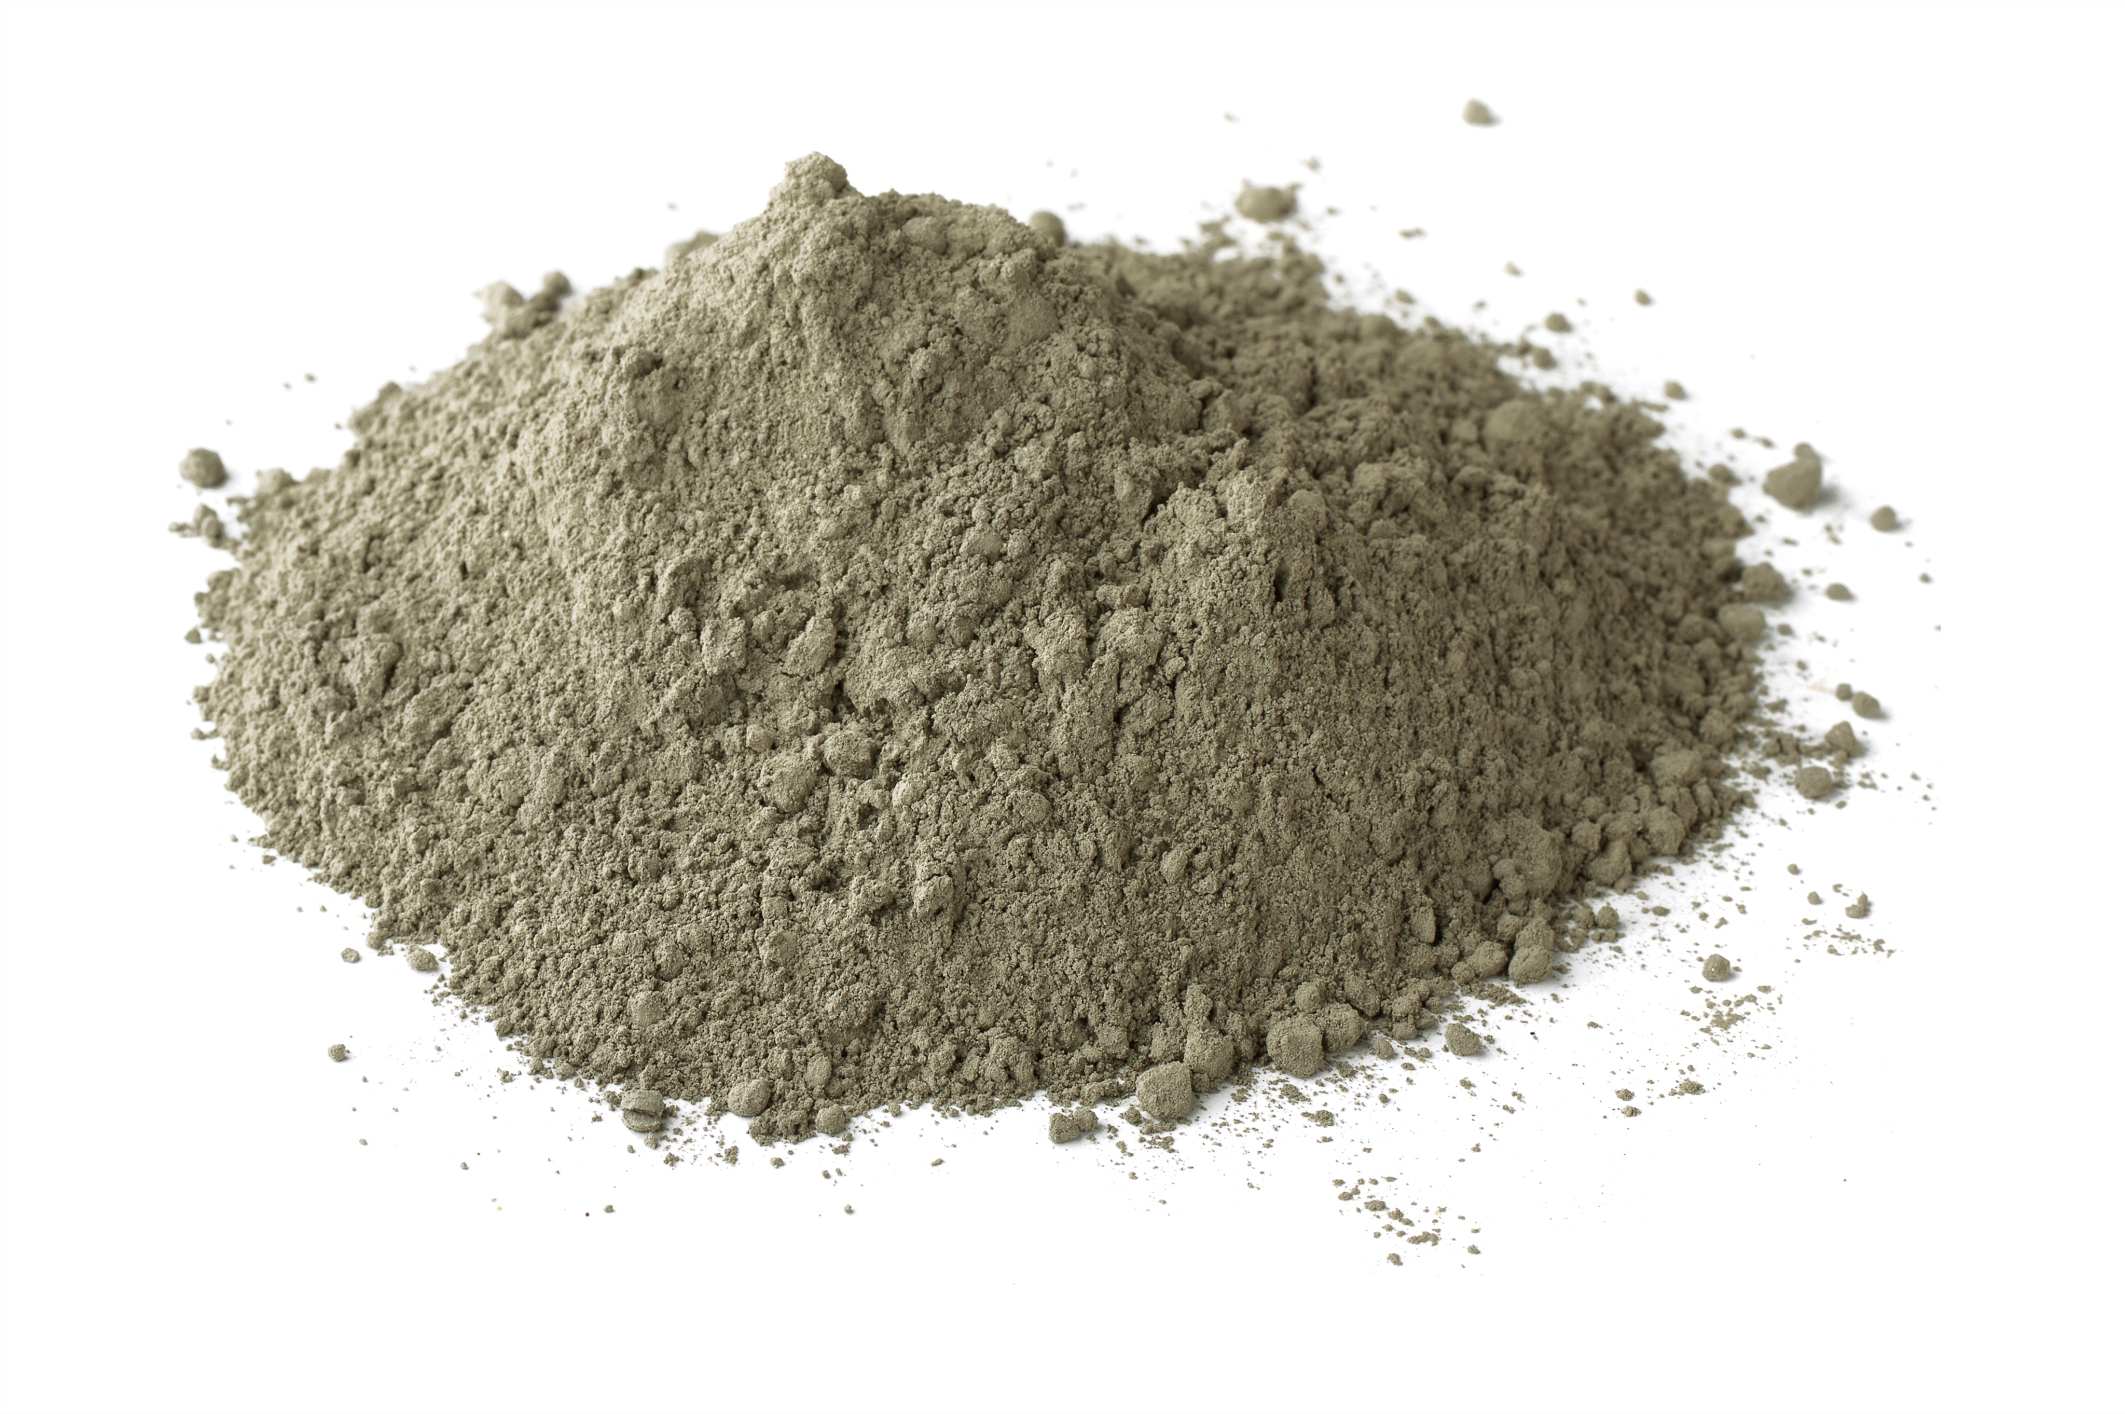
\includegraphics[width=10cm]{figuras/Cimento-Portland.jpg}
		}{
			\Fonte{\citeonline{Teste2021}.}
		}	
	\end{figure}

\section{Composição química geral do cimento}


% dar um contexto. Gráficos e Tabelas servem como apoio ao texto, apenas.

A tabela \ref{tab:componentes-cimento} apresenta os principais componentes presentes na composição química do cimento, suas respectivas fórmulas, intervalo de percentuais em relação à composição total e que papeis possuem no produto final. Segundo \cite{composition-portland-cement}, os cimentos Portland são geralmente compostos por 95\% de clínquer de cimento e 5\% de di-hidrato de sulfato de cálcio, que atua como regulador do tempo de pega.

\begin{table}[h!]
    \centering
    \Caption{\label{tab:componentes-cimento} Componentes do cimento e suas funcionalidades}
    \UFCtab{}{
        \begin{tabular}{|m{4cm}|m{4cm}|m{2cm}|m{6cm}|}
            \toprule
            \textbf{NOME DO COMPOSTO} & \textbf{FÓRMULA/ ABREVIATURA} & \textbf{\% NO CIMENTO} & \textbf{FUNCIONALIDADE} \\ 
            \midrule \midrule
            Silicato tricálcico & (CaO)$_3$SiO$_2$/C$_2$S & 45-75\% & Elevada velocidade de hidratação; responsável pela resistência e pelo endurecimento do cimento. \\ 
            \midrule
            Silicato dicálcico & (CaO)$_2$SiO$_2$/C$_3$S & 7-35\% & Contribuição significativa nas resistências mecânicas do cimento a longo prazo. \\ 
            \midrule
            Aluminato tricálcico & (CaO)$_3$Al$_2$O$_3$/C$_3$A & 0-13\% & Ocorre normalmente em cimentos aluminosos tendo formação decorrente das condições de umidade no processo de resfriamento. \\ 
            \midrule
            Ferroaluminato tetracálcico & (CaO)$_4$Al$_2$O$_3$Fe$_2$O$_3$/C$_4$AF & 0-18\% & Supõe-se que seja a composição mais estável utilizada para representar a solução sólida como um todo; imprime resistência à corrosão química do cimento. \\ 
            \bottomrule
        \end{tabular}
    }{
    \Fonte{\cite{Pinheiro2010}}
}
\end{table}


 % Falar sobre a composição dos materiais. Uma seção para cada (argila, calcário, clínquer, etc)

\section{Processo produtivo}

% Agora, falar sobre todo o processo produtivo.....

Temos o processo de produção do cimento Portland como uma série de ações que necessitam de boa coordenação e qualidade para garantir um material de excelência nos aspectos de uso esperados. De forma macro, esse processo se divide nas seguintes etapas: obtenção da matéria prima; pré-homogeneização; moagem de cru; torre de ciclones; clínquer; resfriamento e armazenamento; moagem; e por fim, estocagem.

        \begin{figure}[h!] 
   	    \captionsetup{width=16cm}%Da mesma largura que a figura
		\Caption{\label{fig:fluxograma-processo} Fluxograma do processo produtivo do cimento Portland.}
		\UFCfig{}{
			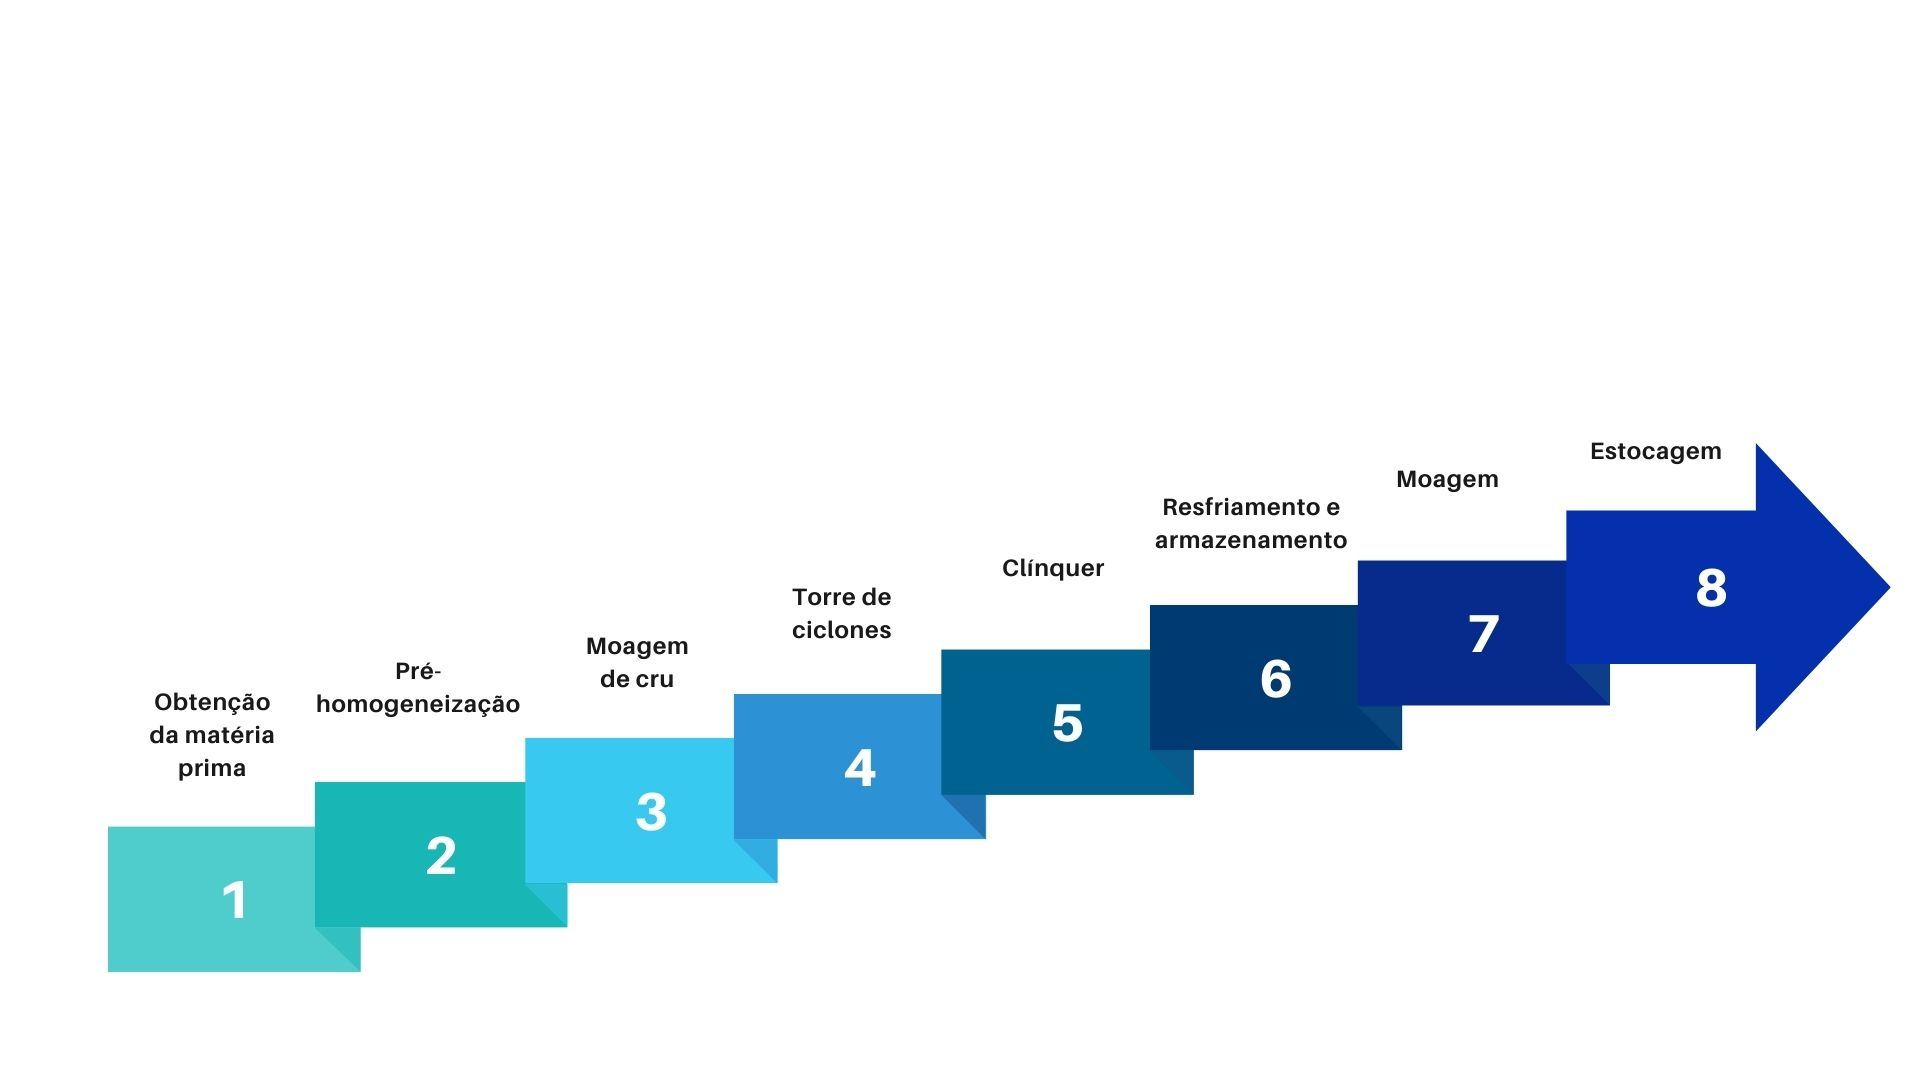
\includegraphics[width=16cm]{figuras/Fluxograma processo produtivo.jpg}
		}{
			\Fonte{\cite{Autor2024}.}
		}	
	\end{figure}


 \pagebreak

 \subsection{Extração da matéria prima e pré-homogeneização}

A etapa inicial na produção do cimento, consiste na extração de calcário e argila diretamente das minas. Em seguida, essas matérias-primas passam pela fase de pré-homogeneização, cujo propósito é o de reduzir os efeitos da composição irregular dos materiais extraídos \cite{Andre2011}. Para realizar o processo de homogeneização, geralmente é aplicado o método Chevron, no qual a matéria-prima é depositada pela empilhadeira formando uma pilha através de movimentos ida e volta, essa ação se repete com a formação de várias camadas com diferentes composições, todas devem possuir mesma espessura. Simultaneamente o material passa pela retomadora, onde a pilha formada será cortada transversalmente por um desagregador removendo as camadas formadas, a retomadora homogeneíza e transporta o material até o centro da pré-homo, onde será levado por uma correia subterrânea até os silos dosadores do calcário \cite{Carvalho2023}.

 	\begin{figure}[h!] 
   	    \captionsetup{width=16cm}%Da mesma largura que a figura
		\Caption{\label{fig:metodo-chevron} Imagem representativa do método Chevron.}
		\UFCfig{}{
			\includegraphics[width=16cm]{figuras/método chevron.jpg}
		}{
			\Fonte{\citeonline{FLSMIDTH2008}.}
		}	
	\end{figure}

 \pagebreak

O material proveniente da pré-homo é transportado até o silo dosador, equipamento
que irá armazenar e dosar a matéria-prima, nele está inserido um dispositivo de dosagem que
permite controlar a quantidade de material que deve seguir para o moinho de cru, esta etapa é
importante para a formação de uma farinha de boa qualidade \cite{Carvalho2023}.

 	\begin{figure}[h!] 
   	    \captionsetup{width=16cm}%Da mesma largura que a figura
		\Caption{\label{fig:silo-dosador} Silo dosador.}
		\UFCfig{}{
			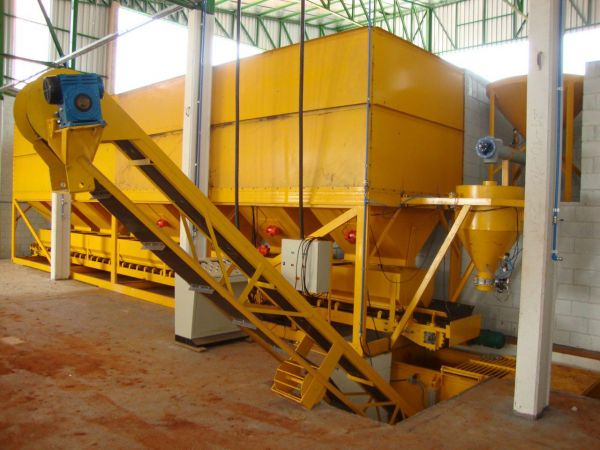
\includegraphics[width=16cm]{figuras/silo-dosador.jpg}
		}{
			\Fonte{\cite{Metallmax}.}
		}	
	\end{figure}

\pagebreak

 \subsection{Moagem de cru}

O argical (mistura de calcário/argila) é empilhado na pilha de estoque da pré homogeneização. Após a pré-homogeneização, segue para o britador secundário. Aquele material que ficou acima de 0,050m segue para o moinho (pode ser de bolas ou vertical) \cite{Andre2011}. O moinho de
cru é um dos principais equipamentos da produção, este que é também chamado de moinho de
rolos vertical, possui 4 rolos sobrepostos em uma mesa giratória que fazem compressão do
material, recebe constantemente a alimentação proveniente dos silos dosadores no centro da
mesa, promovendo atuação da força centrífuga que arrasta o material para as extremidades.
No processo é injetado uma quantidade de água para que o material ao cair no prato não
espalhe, retardando o processo e reduzindo a vibração do equipamento, também existe entrada
de ar quente para reduzir a umidade da farinha, esse ar é proveniente dos gases quentes do
forno que entram no moinho através de um exaustor. O material é então moído e
homogeneizado dentro do moinho até obter uma granulometria menor e uma finura
específica, esta farinha irá passar por um separador, os materiais finos serão separados dos
grossos que retornarão ao sistema para serem moídos novamente \cite{Carvalho2023}.

 	\begin{figure}[h!] 
   	    \captionsetup{width=16cm}%Da mesma largura que a figura
		\Caption{\label{fig:rolo-vertical} Moinho Rolos Vertical.}
		\UFCfig{}{
			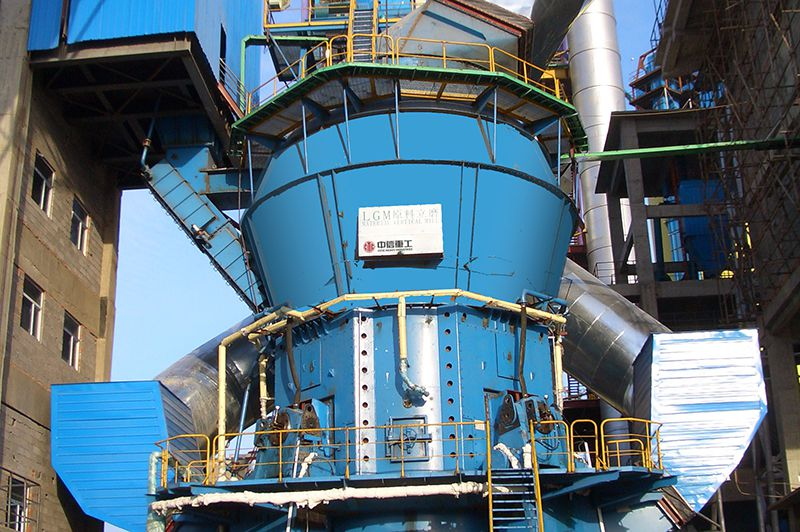
\includegraphics[width=16cm]{figuras/vertical-roller-mill_01.jpg}
		}{
			\Fonte{\cite{CITICHEAVYINDUSTRIES}.}
		}	
	\end{figure}

 \pagebreak

Depois o material se torna uma farinha fina (farinha de cru) e segue para o silo para ser armazenado \cite{Andre2011}. O silo de armazenamento tem como função garantir alimentação contínua do forno, homogeneizar toda farinha presente constantemente e armazenar esse material \cite{Carvalho2023}.

 	\begin{figure}[h!] 
   	    \captionsetup{width=6cm}%Da mesma largura que a figura
		\Caption{\label{fig:silo-armazenamento} Silo de armazenamento.}
		\UFCfig{}{
			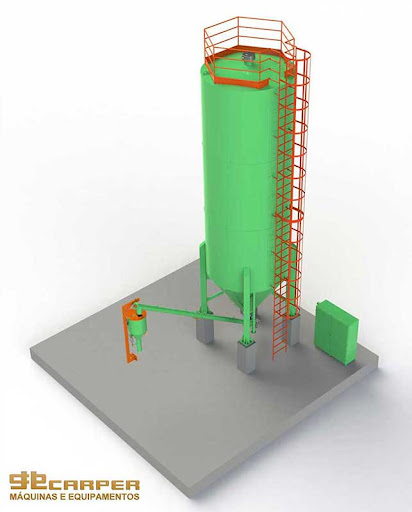
\includegraphics[width=6cm]{figuras/silo-armazenamento.jpg}
		}{
			\Fonte{\cite{CARPER}.}
		}	
	\end{figure}

 \pagebreak

\subsection{Torre de ciclones}

Quando a farinha entra na primeira etapa da torre do ciclone, a temperatura que é de 45ºC a 70ºC aumenta para 440ºC, na segunda etapa da torre de ciclone, atinge de 650ºC. Quando a farinha entra na terceira etapa a temperatura está a 770ºC. Com 900Cº na quarta etapa, o material está no ponto ideal para ser clinquerizado. A farinha aquecida entra no forno para ser cozida por uma chama que pode chegar a uma temperatura de 2000°C \cite{Andre2011}. A torre tem função de pré-aquecer, separar, secar e pré-calcinar a farinha alimentada, que nesta etapa é denominada de farinha produzida. Por meio da recirculação de gás quente advindo do forno, a torre de ciclones promove o transporte da farinha, devido a diferença de temperatura entre o gás e o sólido ocorre a troca de calor, o ciclone separa o gás do sólido, para que a farinha entre no forno e o gás aqueça os outros estágios, dessa forma é feita a retirada da umidade do material e o pré aquecimento. A farinha é alimentada através do duto de ascensão no segundo ciclone e é transportada até o primeiro ciclone, neste trecho os fluxos estão de forma concorrente, ao entrar no ciclone ocorre a separação do gás e da farinha, os gases sobem pelo duto de imersão e a farinha desce, encontrando no estágio inferior gases mais quentes em fluxo contracorrente \cite{Carvalho2023}.

% imagem torre de cliclone

\subsection{Clínquer}

O produto final, clínquer, sai do forno com uma temperatura em torno de 1450ºC e é resfriado com recuperação do calor, é armazenado em um galpão, seguindo para a moagem. Quando o material está sendo moído adicionam-se escória, gesso e material pozolânico a fim de fabricar os diferentes tipos de cimento portland \cite{Andre2011}.

\subsubsection{Compostos do Clínquer}

Segundo \cite{Gobbo2003}, os constituintes do clínquer Portland podem ser subdivididos em três grupos:

\begin{itemize}
    \item Os silicatos cálcicos, são cristais gerados nas últimas etapas do processo de clinquerização e que não sofrem fusão durante sua formação;
    \item A fase intersticial, que representa a fase fundida na temperatura de clinquerização correspondente a temperatura de cristalização dos silicatos, sendo constituída por aluminatos e ferro-aluminatos cálcicos
    \item O terceiro grupo se refere a alguns compostos menos frequentes como o periclásio (MgO), cal livre (CaO), langbeinita {K2Ca2(SO4)3), aphititalita {K3Na(SO4)2}, arcanita {K2SO4, entre outros.
\end{itemize}

\section{Principais fatores que influenciam a vibração}

% identificar quem são as variáveis que coloquei abaixo dentro do processo produtivo passado pela Rose. Talvez marcar uma reunião para saber identificar quem são essas variáveis, onde elas se encaixam no processo produtivo.

Segundo \cite{Zhu2019} e \cite{Hou2022}, os principais fatores que afetam a vibração em um moinho vertical, são os seguintes:

\begin{itemize}

\item Taxa de Alimentação (t/h): A quantidade de material alimentado no moinho deve ser controlada. Taxas de alimentação muito altas ou baixas podem desestabilizar a espessura da camada de moagem, causando vibrações. A alimentação inconsistente pode levar a flutuações na pressão e no fluxo de material.

\item Propriedades do Material: Incluem tamanho das partículas, teor de umidade e dureza dos materiais. Materiais com propriedades variáveis podem alterar a resistência ao rolamento e a formação da camada de moagem, provocando variações na vibração.

\item Espessura da Camada de Moagem: Manter uma espessura consistente da camada de moagem é crucial. Espessuras inconsistentes da camada podem resultar em vibrações. Fatores que afetam isso incluem a taxa de alimentação, o tamanho das partículas e a presença de objetos estranhos.

\item Velocidade da Mesa: Variações podem afetar a eficiência e a estabilidade da moagem.
Altura do Anel de Barragem: Configurações incorretas podem levar à formação inadequada da camada de moagem.

\item Eficiência do Separador: Uma eficiência ruim pode levar a uma circulação interna excessiva de materiais finos, aumentando a vibração.

\item Fluxo de Ar/Gás: Fluxo inadequado de ar através do anel de bicos pode causar flutuações na pressão e na estabilidade.

\item Condição Mecânica: O desgaste dos componentes internos, como rolos e mesas de moagem, pode levar ao aumento da vibração. A manutenção regular desses componentes é essencial para minimizar vibrações.

\item Controle de Temperatura: As temperaturas de entrada e saída do moinho devem ser controladas para evitar superaquecimento, o que pode desestabilizar o sistema e aumentar a vibração. A insuficiente injeção de água para resfriamento ou temperaturas de entrada muito altas podem contribuir para o problema.

\item Sistema Hidráulico: A manutenção adequada do sistema hidráulico que controla a pressão de moagem é essencial para evitar vibrações devido a forças de moagem flutuantes. Parâmetros como a força de moagem, pressão de nitrogênio e a condição dos cilindros hidráulicos são críticos.

\end{itemize}


\section{OBJETIVOS E JUSTIFICATIVA DO TRABALHO}

Este capítulo mostra o principal objetivo do trabalho e os objetivos específicos. Além disso, também descreve-se as justificativas para realização deste trabalho.

\subsection{Objetivo geral}

Contribuir para o controle de vibrações em moinhos de rolos verticais por meio do entendimento das principais variáveis que influenciam esse fenômeno para, posteriormente, aplicar um modelo preditivo utilizando técnicas de aprendizagem profunda, especificamente redes neurais, possibilitando intervenções mais precisas e eficientes para a mitigação das vibrações em um sistema de inteligência artificial. 

\subsection{Objetivos específicos}

\begin{itemize}

\item Coletar e tratar dados da operação.
\item Entender a importância das variáveis na vibração e como se correlacionam.
\item Desenvolver e aplicar um modelo de redes neurais, visando aumento da previsibilidade do comportamento dos moinhos em relação à vibração.

\end{itemize}

    ---------------

Alguns autores preferem fazer uma ``fundamentação teórica'' no segundo capítulo, outros, preferem fazer uma ``revisão da literatura''. Entretanto, isto é particular de cada trabalho e o autor deve escolher o título mais adequado para o capítulo. Consultar o orientador é importante para determinar o título apropriado  \cite{lamport1986latex}.



Evite começar da seção secundária, ou seja, não passe direto do título do capítulo para o título da seção secundária. Escreva um texto para introduzir as seções subsequentes. Lembre-se de utilizar primeira letra maiúscula quando estiver se referindo a um objeto com numeração específica como capítulo, seção, subseção, figura, tabela, quadro, equação, normalmente, se escreve a primeira letra maiúscula da palavra do objeto seguido do \textit{label}. Por exemplo, a Seção \ref{sec:citacoes} explica como fazer citações bibliográficas. Observe no código fonte deste texto como foi feita a referência cruzada. Isso permite enumerar a seção do modo automático o que facilita caso novas seções sejam criadas.  

\section{Citações bibliográficas}\label{sec:citacoes}

    Esta frase mostra como citar um livro sobre descargas atmosféricas \cite{rakov2003lightning}. Também podem ser citados \textit{sites} como \citeonline{elat2015densidade}. Você precisa escrever o código da referência no arquivo "referencia.bib" dentro da pasta "elementos-pos-textuais". Veja esse, onde estão alguns exemplos que já foram testados.        

    Referenciando outro livro \cite{LangtangenLogg2017}. Texto texto texto texto texto texto texto texto texto texto texto texto texto texto texto texto texto texto texto. Texto texto texto texto texto texto texto texto texto texto texto texto texto texto texto texto texto texto texto. Texto texto texto texto texto texto texto texto texto texto texto texto texto texto texto texto texto texto texto. Texto texto texto texto texto texto texto texto texto texto texto texto texto texto texto texto texto texto texto.

    Referenciando outro site \nocite{secretaria1999}(SÃO PAULO, 1999). Neste caso, foi utilizado o comando \verb=\nocite{}=
    que faz com que a referência aparaça e em seguida foi escrito manualmente (SÃO PAULO, 1999). Esse recurso foi utilizado porque se existem particularidades ao citar um estado. E não havia uma macro elaborada para esta citação. Assim, sempre que o estila da citação tiver uma particularidade não contemplada pelo nosso modelo, é possível utilizar este recurso manual.
    
    Texto texto texto texto texto texto texto texto texto texto texto texto texto texto texto texto texto texto texto. Texto texto texto texto texto texto texto texto texto texto texto texto texto texto texto texto texto texto texto. Citando uma norma \cite{NBR10520:2002}.
        
    Citação de duas referências que concordam entre si \cite{Almeida2018,Gondim2017}. Texto texto texto texto texto texto texto texto texto texto texto texto texto texto texto texto texto texto texto. Texto texto texto texto texto texto texto texto texto texto texto texto texto texto texto texto texto texto texto. Texto texto texto texto texto texto texto texto texto texto texto texto texto texto texto texto texto texto texto. Texto texto texto texto texto texto texto texto texto texto texto texto texto texto texto texto texto texto texto texto texto texto texto texto texto texto. Citando um manual \nocite{manuais1989}(SÃO PAULO, 1989). 
        
    Outro tipo de citação é a citação literal ou direta com mais de três linhas. Este tipo de citação deve ser destacada com recuo de $4~cm$ da margem esquerda com letra menor (tamanho 10), sem aspas e com espaçamento simples.  Para exemplificar esse tipo de citação, considere a afirmação de \citeonline[p.~98]{feitosa2016}:
    \begin{citacao}
        A cultura é o processo através do qual o homem cria o algo onde antes imperava o nada. Esse algo é toda complexidade de criações simbólicas, de sentidos e significados que damos às coisas e ao mundo. Um ``algo'' que não se sustenta se não se entender os processos culturais como mecanismos de mediação entre nós e os fenômenos. Assim, mais do que apenas um elemento da comunicação, a mediação é, por excelência, cultural. As diversas modalidades de mediação são apenas sotaques diferenciados dessa mediação cultural. Assim é a mediação informacional.
    \end{citacao}
        
    A afirmação do parágrafo anterior também pode ser reproduzida com a citação na final como mostra o exemplo a seguir: 
    \begin{citacao}
        A cultura é o processo através do qual o homem cria o algo onde antes imperava o nada. Esse algo é toda complexidade de criações simbólicas, de sentidos e significados que damos às coisas e ao mundo. Um “algo” que não se sustenta se não se entender os processos culturais como mecanismos de mediação entre nós e os fenômenos. Assim, mais do que apenas um elemento da comunicação, a mediação é, por excelência, cultural. As diversas modalidades de mediação são apenas sotaques diferenciados dessa mediação cultural. Assim é a mediação informacional. \cite[p.~98]{feitosa2016}.
    \end{citacao}
        
%Mais exemplos e opções de citações podem ser encontradas em:
%        https://en.wikibooks.org/wiki/LaTeX/Bibliography_Management
%        https://github.com/cfgnunes/latex-cefetmg/blob/master/latex-cefetmg/03-elementos-pos-textuais/apendices.tex            

\section{Inserindo figuras}\label{sec:figuras}
    
    A Figura \ref{fig:reitoria} apresenta a fotografia da reitoria da Universidade Federal do Ceará. Observe a estrutura do código para ver como inserir figuras. No título, comece especificando o tipo de figura. Por exemplo, fotografia, desenho, diagrama, fluxograma, gráfico e etc. O espaçamento entre linhas no título é de $1~pt$ (espaçamento simples), apenas a primeira letra da frase é maiúscula. As demais palavras são escritas com letra maiúsculas somente quando são nomes próprios e não há ponto final. 
    
    As margens do título da figura são delimitadas pelo tamanho da figura. Por isso, procure ajustar o tamanho da figura para preencher a largura delimitada pelas margens esquerda e direita da página que possui $16~cm$ de largura. Não esqueça de indicar fonte da figura. O autor deve evitar deixar figuras pequenas menores do que $7~cm$ de largura.
    
    A posição da figura deve ser o mais próximo logo após ter sido chamada no texto (a figura nunca deve aparecer antes de ter sido anunciada no texto). 
    
    %troque h pelo b ou t para mudar a posição da figura.
 	\begin{figure}[h!] 
   	    \captionsetup{width=16cm}%Da mesma largura que a figura
		\Caption{\label{fig:reitoria} Fotografia da reitoria da Universidade Federal do Ceará}
		\UFCfig{}{
			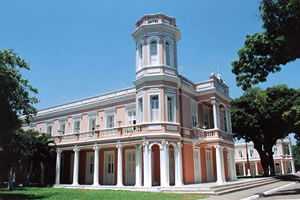
\includegraphics[width=16cm]{figuras/exemplo-1}
		}{
			\Fonte{\citeonline{UFC2012}.}
		}	
	\end{figure}
	
    Texto1 texto texto texto texto texto texto texto texto texto texto texto texto texto texto texto texto texto texto texto texto texto texto texto texto texto texto texto texto texto texto texto texto texto texto texto texto texto texto texto texto texto texto texto texto1.

    Texto2 texto texto texto texto texto texto texto texto texto texto texto texto texto texto texto texto texto texto. Texto texto texto texto texto texto texto texto texto texto texto texto texto texto texto texto texto texto texto2.

    Texto3 texto texto texto texto texto texto texto texto texto texto texto texto texto texto texto texto texto texto. Texto texto texto texto texto texto texto texto texto texto texto texto texto texto texto texto texto texto texto3.

    Texto4 texto texto texto texto texto texto texto texto texto texto texto texto texto texto texto texto texto texto. Texto texto texto texto texto texto texto texto texto texto texto texto texto texto texto texto texto texto texto4.

    A Figura \ref{fig:sondas} texto texto texto texto texto texto texto texto texto texto texto texto texto texto texto texto texto texto texto. Texto texto texto texto texto texto texto texto texto texto texto texto texto texto texto texto texto texto texto3.

	\begin{figure}[h!]
		\centering
		\captionsetup{width=14cm}%Da mesma largura que a figura
		\Caption{\label{fig:sondas} Gráfico da atmosfera superior}	
		\UFCfig{}{
			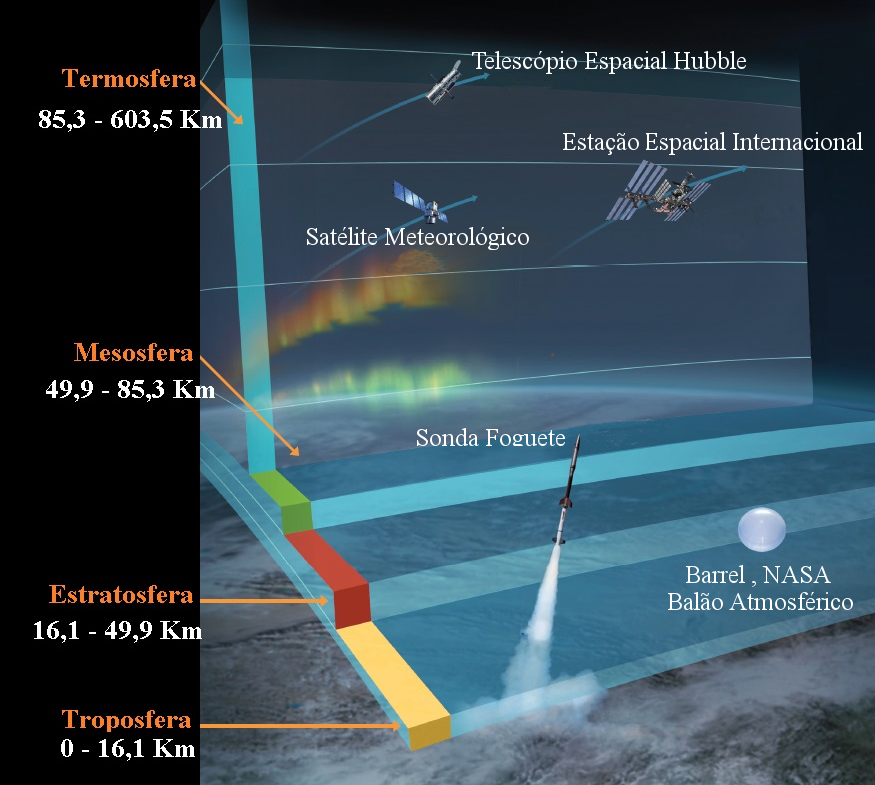
\includegraphics[width=14cm]{figuras/sondas}
		}{
			\Fonte{adaptado da \citeonline{NASA2016}.}}	
	\end{figure}

    Texto5 texto texto texto texto texto texto texto texto texto texto texto texto texto texto texto texto texto texto texto texto texto texto texto texto texto texto texto texto texto texto texto texto texto texto texto texto texto texto texto texto texto texto texto texto5.

    Texto6 texto texto texto texto texto texto texto texto texto texto texto texto texto texto texto texto texto texto texto texto texto texto texto texto texto texto texto texto texto texto texto texto texto texto texto texto texto texto texto texto texto texto texto texto5.

    Texto7 texto texto texto texto texto texto texto texto texto texto texto texto texto texto texto texto texto texto texto texto texto texto texto texto texto texto texto texto texto texto texto texto texto texto texto texto texto texto texto texto texto texto texto texto texto texto texto texto texto texto texto texto texto texto texto texto texto texto texto texto texto texto texto6.

    Evite terminar seções, capítulos e etc com figura. Procure escrever mais.

\section{Inserindo tabelas}\label{sec:tabelas}
    
    A Tabela \ref{tab:exemplo-1}... texto texto texto texto texto texto texto texto texto texto texto texto texto texto texto texto texto texto texto. Texto texto texto texto texto texto texto texto texto texto texto texto texto texto texto texto texto texto texto.
	
	\begin{table}[!h]
	\captionsetup{width=7cm}%Deixe da mesma largura que a tabela
	\caption{\label{tab:exemplo-1} Um Exemplo de tabela alinhada que pode ser longa ou curta}%
	\IBGEtab{}{%
		\begin{tabular}{ccc}
			\toprule
			Nome & Nascimento & Documento \\
			\midrule \midrule
			Maria da Silva & 11/11/1111 & 111.111.111-11 \\
			Maria da Silva & 11/11/1111 & 111.111.111-11 \\
			Maria da Silva & 11/11/1111 & 111.111.111-11 \\
			\bottomrule
		\end{tabular}%
	}{%
	\Fonte{o autor.}%
	\Nota{esta é uma nota, que diz que os dados são baseados na
		regressão linear.}%
	\Nota[Anotações]{uma anotação adicional, seguida de várias outras.}%
    }
    \end{table}

	%\begin{table}[h!]	
	%	\centering
	%	\Caption{\label{tab:exemplo-1} Exemplo de tabela}	
	%	\UFCtab{}{
	%		\begin{tabular}{cll}
	%			\toprule
	%			Ranking & Exon Coverage & Splice Site Support \\
	%			\midrule \midrule
	%			E1 & Complete coverage by a single transcript & Both splice sites\\
	%			E2 & Complete coverage by more than a single transcript & Both splice sites\\
	%			E3 & Partial coverage & Both splice sites\\
	%			E4 & Partial coverage & One splice site\\
	%			E5 & Complete or partial coverage & No splice sites\\
	%			E6 & No coverage & No splice sites\\
	%			\bottomrule
	%		\end{tabular}
	%	}{
	%	\Fonte{elaborado pelo autor.}
	%}
	%\end{table}

\subsection{Exemplo de subseção} \label{sec:ex_sec}
	
    Texto texto texto texto texto texto texto texto texto texto texto texto texto texto texto texto texto texto texto texto texto texto texto texto texto texto texto texto texto texto texto texto texto texto texto texto texto texto texto texto texto texto texto texto texto.

    %acrlong{DATASUS},\acrlong{DNV},\acrlong{DO},\acrlong{ESF},\acrlong{IBGE},\acrlong{MFC},\acrlong{MI},\acrlong{MS},\acrlong{NV},\acrlong{ODM},\acrlong{OI},\acrlong{OMS},\acrlong{ONU},\acrlong{PNI},\acrlong{PSF},\acrlong{RIPSA},\acrlong{RN},\acrlong{SIM},\acrlong{SINASC},\acrlong{SUS},\acrlong{TMI},\acrlong{TMMFC}


    \begin{itemize}
	    \item Integer non lacinia magna. Aenean tempor lorem tellus, non sodales nisl commodo ut
	    \item Proin mattis placerat risus sit amet laoreet. Praesent sapien arcu, maximus ac fringilla efficitur, vulputate faucibus sem. Donec aliquet velit eros, sit amet elementum dolor pharetra eget
	    \item Integer eget mattis libero. Praesent ex velit, pulvinar at massa vel, fermentum dictum mauris. Ut feugiat accumsan augue, et ultrices ipsum euismod vitae
	    \begin{itemize}
		    \item Integer non lacinia magna. Aenean tempor lorem tellus, non sodales nisl commodo ut
		    \item Proin mattis placerat risus sit amet laoreet.
	    \end{itemize}
    \end{itemize}

\subsection{Uso de siglas} \label{sec:siglas}

    Para utilizar siglas, primeiro defina a sigla no arquivo "lista-de-abreviaturas-e-siglas"~ dentro da pasta "1-pre-textuais" com o comando 
    \begin{verbatim}
        \newacronym{ABNT}{ABNT}{Associação Brasileira de Normas Técnicas}
    \end{verbatim}
    Depois chame a sigla com o comando:
    \begin{verbatim}
        \gls{ABNT}
    \end{verbatim}
    Fica assim: \gls{ABNT}. A primeira vez que o comando é usado para uma determinada sigla, aparece o significado por extenso da sigla com a sua abreviação em seguida. A partir da segunda vez que o comando para uma determinada sigla é usado, aparace apenas a sigla. Por exemplo: \gls{ABNT}.  
    
    Veja o código fonte de outros exemplos: Teste de siglas \gls{TEST}, outros exemplos de siglas: \gls{DA}, \gls{MCEG}. 
    Repare que sempre as siglas estão sendo definidas primeiramente no arquivo ``lista-de-abreviaturas-e-siglas''.